% 物理352–357／印刷329–334；习题31–69.
\subsection*{\hyperref[sec:5]{第5章}主题的习题}
\begin{exercise}\label{ex:31}
$\spadesuit$ 设 $X$ 为 Polish 度量空间，$\mu_n,\mu\in\mathscr P_1(X)$ 为 $X$ 上的概率测度，且对每个 $\phi\in\Lip_1(X)$，有 $\int\phi\dd\mu_n\to\int\phi\dd\mu$. 证明，对每个 $\phi\in C_b(X)$，都有 $\int\phi\dd\mu_n\to\int\phi\dd\mu$.
\end{exercise}

\begin{exercise}\label{ex:32}
证明，对任意紧集 $\Sigma\subset\Omega$ 及满足 $f\geq0$、$\int_\Omega f(x)\dd x=1$ 的任意密度 $f\in L^1(\Omega)$，有以下等式：
\[
\begin{aligned}
\int d(x,\Sigma)f(x)\dd x
&=\min\{W_1(f,\nu):\nu\in\mathscr P(\Sigma)\}\\
&=\min\{|\mathbf w|(\Omega):\mathbf w\in\mathscr M_{\mathrm{div}}^d(\Omega),\ \spt(\nabla\cdot\mathbf w-f)\subset\Sigma\}.
\end{aligned}
\]
若改为考虑 $p>1$ 时的 $\int d(x,\Sigma)^pf(x)\dd x$，能说些什么?
\end{exercise}

\begin{exercise}\label{ex:33}
设 $\gamma\in\Pi(\mu,\nu)$ 是分别位于两个紧空间 $X$ 和 $Y$ 上的概率测度之间的运输方案. 设 $\mu_n\rightharpoonup\mu$、$\nu_n\rightharpoonup\nu$ 为两个弱收敛的概率测度序列. 证明，存在序列 $\gamma_n\in\Pi(\mu_n,\nu_n)$，使 $\gamma_n\rightharpoonup\gamma$. 推出，对任意一致收敛于 $c$ 的费用序列 $c_n$，有 $\mathscr T_{c_n}(\mu_n,\nu_n)\rightharpoonup\mathscr T_c(\mu,\nu)$.
\end{exercise}

\begin{exercise}\label{ex:34}
设 $\Omega\subset\R^d$ 光滑且紧，$V$ 是一个算子，将每个概率测度 $\varrho\in\mathscr P(\Omega)$ 对应到向量场 $V[\varrho]:\Omega\to\R^d$，具有以下性质：对每个 $\varrho$，$V[\varrho]$ 为 Lipschitz 连续，且满足 $\Lip(V[\varrho])\leq C$（常数 $C$ 不依赖于 $\varrho$），并在 $\partial\Omega$ 上有 $V[\varrho]\cdot\mathbf n=0$；映射 $\varrho\mapsto V[\varrho]$ 在以下意义下为 Lipschitz 连续：对每个 $\varrho,\mu$，有 $\|V[\varrho]-V[\mu]\|_{L^\infty}\leq CW_2(\varrho,\mu)$. 考虑初始 Cauchy 条件为 $\varrho_0\ll\mathscr L^d$ 的方程 $\partial_t\varrho+\nabla\cdot(\varrho V[\varrho])=0$. 证明，任意解 $\varrho_t$ 在 $t>0$ 时保持绝对连续，并证明解的唯一性.
\end{exercise}

\begin{exercise}\label{ex:35}
$\spadesuit$ 对紧支集测度 $\mu,\nu$，证明等式 $W_\infty(\mu,\nu)=\lim_{p\to\infty}W_p(\mu,\nu)$. 还要证明，对任意序列 $p_n\to\infty$，费用 $|x-y|^{p_n}$ 的最优方案 $\gamma_n$ 至多取子列后，收敛于定义 $W_\infty$ 距离的问题的一个最优方案.
\end{exercise}

\begin{exercise}\label{ex:36}
证明不等式 $d_H(\spt(\mu),\spt(\nu))\leq W_\infty(\mu,\nu)$，其中 $d_H$ 表示 Hausdorff 距离.
\end{exercise}

\begin{exercise}\label{ex:37}
* 是否有以下结论：对 $1\leq p\leq q\leq\infty$，若同一映射 $\mathrm T$ 在 $W_p$ 与 $W_q$ 的定义中都最优，则它在每个 $r\in[p,q]$ 对应的 $W_r$ 定义中也最优?
\end{exercise}

\begin{exercise}\label{ex:38}
证明，若 $f\in W^{1,p}(\Omega)$，$\Omega$ 为凸集，$\mu,\nu\in\mathscr P(\Omega)\cap L^r(\Omega)$，且 $\|\mu\|_{L^r},\|\nu\|_{L^r}\leq C$，则当 $\frac1p+\frac1q+\frac1r=1+\frac1{qr}$ 时，有
\[
\int_\Omega f\dd(\mu-\nu)\leq C^{1/q'}\|\nabla f\|_{L^p(\Omega)}W_q(\mu,\nu).
\]
\end{exercise}

\subsection*{\hyperref[sec:6]{第6章}主题的习题}
\begin{exercise}\label{ex:39}
设 $\Sigma=\{x_1,\ldots,x_N\}\subset\Omega$ 是紧凸区域 $\Omega$ 的一个有限子集. 对每个 $i$，令 $V_i:=\{x\in\Omega:|x-x_i|\leq|x-x_j|\text{ 对所有 }j\}$. 假设 $\Sigma$ 解出问题 $\min\{\int_\Omega d(x,\Sigma)^2\dd x:\#\Sigma\leq N\}$. 证明，对每个 $i$，点 $x_i$ 是 $V_i$ 的重心.
\end{exercise}

\begin{exercise}\label{ex:40}
$\spadesuit$ 对 $A\subset\R^d$，将 $A$ 的极点定义为满足以下条件的点 $x\in A$：$y,z\in A$ 且 $x=(y+z)/2\Longrightarrow y=z$. 设 $K\subset\mathscr M_n(\R)$ 为双随机矩阵集合（即满足 $m_{ij}\geq0$、$\sum_jm_{ij}=\sum_im_{ij}=1$，对所有 $i,j$ 成立的矩阵 $M=(m_{ij})$）. 证明，$k$ 的极点是置换矩阵.
\end{exercise}

\begin{exercise}\label{ex:41}
对 $a\in(\R_+)^n$、$b\in(\R_+)^m$，考虑如下定义的集合 $\Pi(a,b)$：
\[
\Pi=\left\{M\in\mathscr M_{n,m}(\R):m_{ij}\geq0,\ \sum_jm_{ij}=a_i,\ \sum_im_{ij}=b_j\right\}.
\]
证明，$\Pi(a,b)$ 中的每个极点矩阵 $M$ 都满足 $\#\{(i,j):m_{ij}>0\}\leq n+m$.
\end{exercise}

\begin{exercise}\label{ex:42}
设 $\gamma_{ij}^\varepsilon:=p_i^\varepsilon q_j^\varepsilon\eta_{ij}$ 为\eqref{eq:6.3}中近似问题的一个解（见\autoref{sec:6.4.1}）. 假设 $\varepsilon\log(p_i^\varepsilon)$、$\varepsilon\log(q_j^\varepsilon)$ 以及 $\gamma_{ij}^\varepsilon$ 在 $\varepsilon\to0$ 时收敛. 证明，$\varepsilon\log(p_i^\varepsilon)$ 与 $\varepsilon\log(q_j^\varepsilon)$ 的极限是 $\varepsilon=0$ 时极限问题的 Kantorovich 势.
\end{exercise}

\begin{exercise}\label{ex:43}
设 $u$ 为 $\Omega$ 上的光滑函数，$M(x):=\cof(D^2u(x))$. 设 $M^{ij}$ 为 $M$ 的 $(i,j)$ 元，$M_k^{ij}$ 为其关于 $x_k$ 的导数. 证明，对每个指标 $j$，有 $\sum_iM_i^{ij}(x)=0$.
\end{exercise}

\begin{exercise}\label{ex:44}
* $\spadesuit$ 在光滑区域 $\Omega$ 上，考虑形如 $\mathrm T=\nabla u$ 的光滑运输映射 $\mathrm T:\Omega\to\R^d$. 假设 $\mathrm T_\#f=\nu$，其中 $f$ 为 $\Omega$ 上的光滑正密度. 对每个满足 $\nabla\cdot(f\mathbf v)=0$ 且在 $\partial\Omega$ 上 $\mathbf v\cdot\mathbf n=0$ 的向量场 $\mathbf v:\Omega\to\R^d$，考虑该自治向量场的流 $Y_t(x)=y_x(t)$（其中 $y'_x(t)=\mathbf v(y_x(t))$ 且 $y_x(0)=x$），并定义 $\mathrm T_t=\mathrm T\circ Y_t$. 令 $M(S)=\int|S(x)-x|^2f(x)\dd x$. 证明，函数 $j(t)=M(\mathrm T_t)$ 对每个 $\mathbf v$ 均满足 $j''(0)\geq0$，当且仅当 $u$ 为凸函数.
\end{exercise}

\subsection*{\hyperref[sec:7]{第7章}主题的习题}
\begin{exercise}\label{ex:45}
* $\spadesuit$ 证明熵泛函
\[
\mathscr F(\varrho):=\begin{cases}
\displaystyle\int_{\R^d}\varrho(x)\log\varrho(x)\dd x,&\varrho\ll\mathscr L^d,\\
+\infty,&\text{其他情形}
\end{cases}
\]
在 $\mathbb W_1(\R^d)$ 中下半连续. 还要证明，若 $\varrho_n\in\mathscr P_2(\R^d)$，且 $\varrho_n\rightharpoonup\varrho$、$\int|x|^2\dd\varrho_n(x)\leq C$，则 $\mathscr F(\varrho)\leq\liminf_n\mathscr F(\varrho_n)$.
\end{exercise}

\begin{exercise}\label{ex:46}
证明，只要 $\varrho_0,\varrho_1\leq1$ 且 $\Omega$ 凸，问题
\[
\min\left\{\int_0^1\int_\Omega\varrho|\mathbf v|^2\dd x\dd t:
\begin{array}{l}
\partial_t\varrho+\nabla\cdot(\varrho\mathbf v)=0,\ \varrho_t\in\mathscr P(\Omega),\\
\varrho(0)=\varrho_0,\ \varrho(1)=\varrho_1
\end{array}\right\}
\]
与再加上约束 $\varrho_t\leq1$ 的同一问题等价. 再构想一个非凸（但连通）的区域 $\Omega$，使该结论不再成立.
\end{exercise}

\begin{exercise}\label{ex:47}
给定紧凸区域 $\Omega\subset\R^d$ 和 $\nu\in\mathscr P(\Omega)$，证明下述问题有解：
\[
\min\left\{W_1(\varrho,\nu)+\frac12\int\varrho^2(x)\dd x:
\varrho\in L^2(\Omega),\ \varrho\geq0,\ \int\varrho(x)\dd x=1\right\}.
\]
解是否唯一? 写出最优 $\varrho$ 满足的最优性条件，证明 $\varrho\in\Lip_1$，并在 $\Omega=\overline{B(0,5)}$、$\nu=\delta_0$ 时显式求解.
\end{exercise}

\begin{exercise}\label{ex:48}
** 给定 $p>1$，考虑绝对连续概率测度 $g\in\mathscr P(\Omega)$，以及问题 $\min\{W_p(\varrho,g):\varrho\leq f\}$，其中 $f\in L^1(\Omega)$ 为给定的正函数. 证明，存在唯一解，且它形如 $\varrho=\mathbbm1_Ag+\mathbbm1_{A^c}f$.
\end{exercise}

\subsection*{\hyperref[sec:8]{第8章}主题的习题}
\begin{exercise}\label{ex:49}
考虑四阶偏微分方程
\[
\partial_t\varrho+\nabla\cdot(\varrho\nabla(\Delta\varrho))
+\nabla\cdot\left(\frac{\nabla\varrho}{\sqrt\varrho}\right)=0.
\]
这个方程是某个能量在 $\mathbb W_2$ 中的梯度流：这个能量是什么? 还要证明，对应的极小化运动格式在每个时间步需要求解的变分问题（见\eqref{eq:8.3}）都有解.
\end{exercise}

\begin{exercise}\label{ex:50}
设 $V:\R^d\to\R$ 属于 $C^{1,1}$，$\mathscr G:\mathscr P(\R^d)\to\R$ 由 $\mathscr G(\varrho)=\#(\spt(\varrho))$ 定义；设 $\varrho_0\in\mathscr P(\R^d)$ 为具有有限多个原子的纯原子概率测度 $\varrho_0=\sum_{i=1}^Na_i\delta_{x_i^0}$. 证明，当 $\tau$ 较小时（依赖于什么?），极小化问题
\[
\min\left\{\mathscr G(\varrho)+\int V\dd\varrho+\frac{W_2^2(\varrho^0,\varrho)}\tau:
\varrho\in\mathscr P_2(\R^d)\right\}
\]
有唯一解，且形如 $\varrho_1=\sum_{i=1}^Na_i\delta_{x_i^1}$，并满足 $\mathscr G(\varrho_1)=\mathscr G(\varrho_0)$. 推出，$\mathscr G+\mathscr V$ 的极小化运动格式给出与 $\mathscr V$ 相同的极限曲线，并求出这条曲线的方程.
\end{exercise}

\begin{exercise}\label{ex:51}
设 $\varrho_0\in\mathscr P_2(\R^d)$，$x_0$ 为其重心，$\varrho$ 为方程
\[
\partial_t\varrho_t-\nabla\cdot(\varrho_t\mathbf v_t)=0
\]
的一个解，其中 $\mathbf v_t(x)=\int(x-y)\dd\varrho_t(y)$. 令 $E(t):=\int|x-x_0|^2\dd\varrho_t(x)$. 证明 $E'(t)\leq-E(t)$. 对 $t\to\infty$ 时 $\varrho_t$ 的渐近行为，可以得出什么结论?
\end{exercise}

\begin{exercise}\label{ex:52}
设 $V:\R^d\to\R$ 为连续函数，满足 $|V(x)|\leq A+B|x|^2$，其中 $A,B$ 为适当常数；设 $f:\R^+\to\R$ 为凸函数，且 $f'(0)>-\infty$. 定义
\[
F(\varrho)=\int f(\varrho(x))\dd x+\int V(x)\varrho(x)\dd x,
\]
并对 $\varrho_0\in\mathscr P_2(\R^d)$ 考虑
\[
\min\left\{F(\varrho)+\frac{W_2^2(\varrho,\varrho_0)}{2\tau}:
\varrho\in\mathscr P_2(\R^d)\right\}.
\]
证明，当 $\tau$ 较小时，存在唯一解；若 $\varrho_0$ 具有紧支集，则解也具有紧支集.
\end{exercise}

\begin{exercise}\label{ex:53}
考虑 $m>2$ 并定义
\[
F(\varrho)=\int_\Omega\varrho^m-\frac12\int_\Omega|\nabla u_\varrho|^2,
\qquad\text{其中 }u_\varrho\in H_0^1(\Omega)\text{ 满足 }-\Delta u_\varrho=\varrho.
\]
证明
\[
\min\{F(\varrho)+W_2^2(\varrho,\varrho_0):\varrho\in\mathscr P_2(\R^d)\}
\]
有解.
\end{exercise}

\begin{exercise}\label{ex:54}
证明，问题
\[
\min\left\{\int_0^T\int\left(\frac{t^{3/2}}2\varrho|\mathbf v|^2
+\frac{3t^{-1/2}}4|\nabla\varphi|^2\right):
\begin{array}{l}
\partial_t\varrho+\nabla\cdot(\varrho\mathbf v)=0,\\
\Delta\varphi=\varrho-1,\\
\varrho_0=1,\ \varrho_T=\text{给定}
\end{array}\right\}
\]
的最优性条件，至少在形式上给出\eqref{eq:8.27}的方程组.
\end{exercise}

\begin{exercise}\label{ex:55}
给定 $\alpha\in ]0,1[$，证明问题
\[
\min\left\{\int_0^1t^{1+\alpha}|x'(t)|^2+ct^{-1+\alpha}|x(t)-x_0|^2:x(1)=x_1\right\}
\]
有唯一极小点，且满足 $x(0)=x_0$. 证明，对于再加上条件 $x(0)=\widetilde x_0$、其中 $\widetilde x_0\neq x_0$ 的同一问题，不存在极小点.
\end{exercise}

\begin{exercise}\label{ex:56}
考虑环面 $\mathbb T^d$ 上的三元组 $(\varrho_t,\mathbf v_t,\varphi_t)$（以避免边界问题），满足
\[
\int_0^1\int\left(\frac{t^{3/2}}2\varrho|\mathbf v|^2+\frac{3t^{-3/2}}2|\nabla\varphi|^2\right)<+\infty,
\quad\begin{cases}
\partial_t\varrho_t+\nabla\cdot(\varrho_t\mathbf v_t)=0,\\
\Delta\varphi_t=\varrho_t-1,
\end{cases}
\]
并满足 $\|\varrho_t\|_{L^\infty}\leq C$，且 $t\mapsto\varrho_t$ 关于 $W_2$ 在 $]0,1]$ 上连续. 证明，当 $t\to0$ 时，必有 $W_2(\varrho_t,1)\to0$.
\end{exercise}

\subsection*{杂题}
\begin{exercise}\label{ex:57}
对形如 $|x-y|^p$、$p>0$ 的费用，求下图两个测度之间的最优运输映射：
\begin{center}
\begin{minipage}{.18\linewidth}
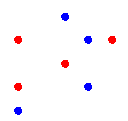
\includegraphics[width=\linewidth]{assets/ex57-points.pdf}
\end{minipage}\qquad
\begin{minipage}{.7\linewidth}
\[
\begin{aligned}
\mu&=\tfrac14(\delta_{(2,3)}+\delta_{(3,2)}+\delta_{(3,0)}+\delta_{(0,-1)}),\\
\nu&=\tfrac14(\delta_{(0,0)}+\delta_{(0,2)}+\delta_{(2,1)}+\delta_{(4,2)}).
\end{aligned}
\]
\end{minipage}
\end{center}
\end{exercise}

\begin{exercise}\label{ex:58}
给出一对 $\R^d$ 上具有紧支集的绝对连续概率测度 $\mu,\nu$，以及连续费用 $c:\R^d\times\R^d\to\R_+$ 的例子，使对应的 Monge 问题不存在最优运输映射.
\end{exercise}

\begin{exercise}\label{ex:59}
在一维中，当 $\mu=\mathscr L^1\restr[0,1]$、$\nu=\frac12\mathscr L^1\restr[-1,1]$ 时，求费用 $c(x,y)=(x^2-y^2)^2$ 的最优运输方案.
\end{exercise}

\begin{exercise}\label{ex:60}
给出一个有界下半连续（但不连续）的费用 $c:\R^d\to\R$，以及两个无原子的紧支集测度 $\mu,\nu\in\mathscr P(\R^d)$ 的例子，使 $\inf(\mathrm{MP})>\min(\mathrm{KP})$.
\end{exercise}

\begin{exercise}\label{ex:61}
* 证明，存在连续映射 $\mathrm T:[0,1]\to[0,1]^2$，满足 $\mathrm T_\#(\mathscr L^1\restr[0,1])=\mathscr L^2\restr[0,1]^2$.
\end{exercise}

\begin{exercise}\label{ex:62}
考虑由 $S(x)=x+a$ 给出的平移 $S:\R^d\to\R^d$.
\begin{enumerate}
\item 证明，对任意测度 $\mu$，$S$ 是 $\mu$ 与 $S_\#\mu$ 之间费用 $c(x,y)=|x-y|^2$ 的最优运输.
\item 对 $c(x,y)=|x-y|$ 证明同样的结论.
\item 若 $\mathrm T$ 为 $\mu$ 与 $\nu$ 之间的最优运输，能否说 $S\circ\mathrm T$ 是 $\mu$ 与 $S_\#\nu$ 之间的最优运输? 分别对 $c(x,y)=|x-y|^2$ 与 $c(x,y)=|x-y|$ 回答.
\item 更一般地，两个最优运输的复合是否仍然最优?
\end{enumerate}
\end{exercise}

\begin{exercise}\label{ex:63}
$\spadesuit$ 证明，若 $J\subset\R$ 是给定的（可以无界的）区间，则 $\mathbb W_p(J)$ 与 $L^p([0,1])$ 的某个闭凸子集等距.
\end{exercise}

\begin{exercise}\label{ex:64}
给定 $g\in L^1([0,1])\cap\mathscr P([0,1])$，证明 $W_2(1,g)=\|1-g\|_{\dot H^{-1}([0,1])}$.
\end{exercise}

\begin{exercise}\label{ex:65}
考虑 $\mu,\nu\in\mathscr P_1(\R^d)$，且 $\int x\dd\mu(x)=\int y\dd\nu(y)=0$. 设 $\gamma$ 是这两个测度之间费用 $c(x,y)=-x\cdot y$ 的最优运输方案，$\mathscr T_c(\mu,\nu)$ 为这一运输费用的最优值. 证明 $\mathscr T_c(\mu,\nu)\leq0$，且 $\spt(\gamma)\subset\{(x,y):x\cdot y\geq\mathscr T_c(\mu,\nu)\}$. 推出，若 $\mu_n\rightharpoonup\mu$ 且 $\int x\dd\mu_n(x)=\int y\dd\nu(y)=0$，则 $\mathscr T_c(\mu,\nu)\geq\limsup_n\mathscr T_c(\mu_n,\nu)$.
\end{exercise}

\begin{exercise}\label{ex:66}
设 $f,g$ 为凸区域 $\Omega$ 上的两个光滑概率密度，$\varphi,\psi$ 是从 $f$ 到 $g$、费用为 $c(x,y)=\frac12|x-y|^2$ 的运输问题的 Kantorovich 势. 证明 $\int\nabla f\cdot\nabla\varphi+\nabla g\cdot\nabla\psi\geq0$. 推出，对 $f,g\in H^1(\Omega)$，同样结论成立.
\end{exercise}

\begin{exercise}\label{ex:67}
证明，热方程 $\partial_t\varrho=\Delta\varrho$ 的两个（光滑）解之间的 $W_2$ 距离随时间递减：
\begin{enumerate}
\item 在有界区域 $\Omega$ 中，采用齐次 Neumann 边界条件；
\item 在 $\R^d$ 中，初值属于 $\mathscr P_2(\R^d)$.
\end{enumerate}
\end{exercise}

\begin{exercise}\label{ex:68}
设 $\mathbf v:[0,T]\times\Omega\to\R^d$ 关于空间为 Lipschitz 连续，且关于时间一致. 通过对两个解之间的 $W_2^2$ 求导，证明带无通量边界条件的 Fokker--Planck 方程 $\partial_t\varrho-\Delta\varrho+\nabla\cdot(\varrho\mathbf v)=0$ 的解，在对每个 $t$ 均属于 $H^1(\Omega)\cap\mathscr P(\Omega)$ 的解类中唯一. 为什么 $H^1$ 是对解正则性的合理假设?
\end{exercise}

\begin{exercise}\label{ex:69}
设 $f:\R^d\to\R$ 为 $C^2$ 严格凸函数，在光滑有界区域 $\Omega$ 上满足 $D^2f\geq\alpha\mathrm I$（某个 $\alpha>0$）. 证明 $\varrho_\infty=ce^{-f}$（其中 $c=(\int e^{-f})^{-1}$）是 $\Delta\varrho+\nabla\cdot(\varrho\nabla f)=0$ 的解. 现在考虑 $\Omega$ 上满足 Neumann 边界条件的方程 $\partial_t\varrho-\Delta\varrho-\nabla\cdot(\varrho\nabla f)=0$ 的任意光滑解，证明当 $t\to\infty$ 时，$W_2(\varrho_t,\varrho_\infty)$ 指数趋于0.
\end{exercise}
